\documentclass[../main.tex]{subfiles}
\graphicspath{{\subfix{../figures/}}}

\begin{document}
\chapter{Introduction}
\label{chapter:intro}
\vspace{-10pt}

\section{Section}
\vspace{-10pt}

\lipsum[1]~\citep{hubel1962receptive}.

\begin{figure}[h!]
  \centering
  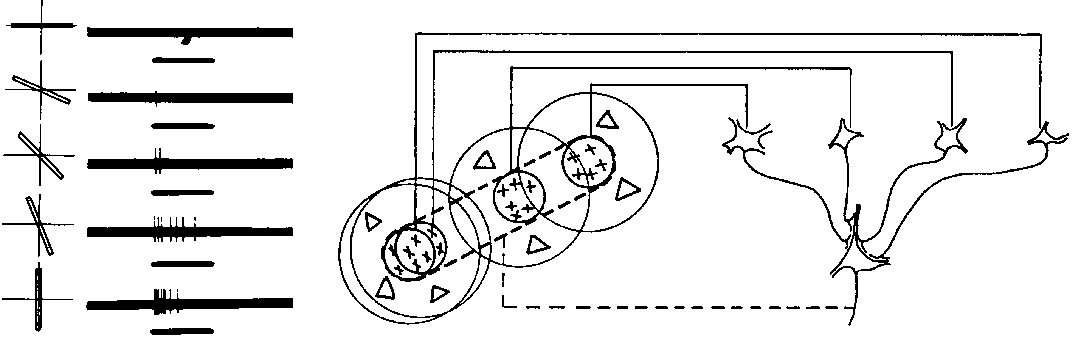
\includegraphics[width=1.\linewidth]{figures/intro_hubel_wiesel.pdf}
  \caption{\textbf{left}: response of an example neuron from a cat's visual cortex to different orientations. \textbf{Right}: Model suggested by \citet{hubel1962receptive} for explaining the organization of simple receptive fields. The figure is adapted from Hubel and Wiesel's original paper~\citep{hubel1962receptive}.}
  \label{fig:intro_hubel_wiesel}
\end{figure}

\biblio
\end{document}